\documentclass[../main.tex]{subfiles}

\begin{document}

\section{Opakování Riemannova integrálu v jedné proměnné}

\begin{figure}[h]
	\centering
	\subfloat[Dolní Riemannova suma]{{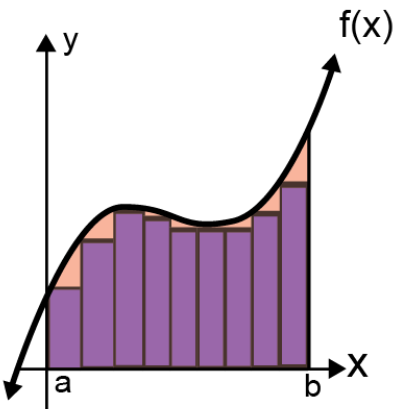
\includegraphics[width=4.6cm]{08-lsum}}}%
	\hfill
	\subfloat[Horní Riemannova suma]{{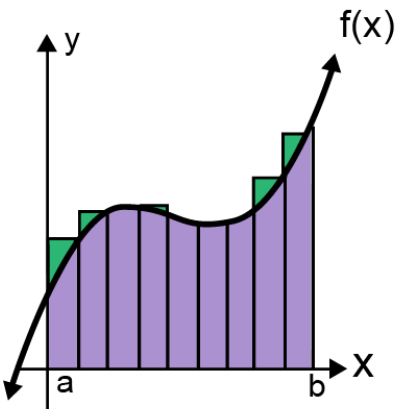
\includegraphics[width=4.6cm]{08-usum}}}%
	\hfill
	\subfloat[Integrál funkce]{{
\includegraphics[width=4.6cm]{08-integral}}}%
	\caption{Geometrický význam Riemannova integrálů jedné proměnné.}
\end{figure}

\begin{definitionnodot}[Rozdělení]
	intervalu $\left<a,b\right>$ je posloupnost 
	\[P : a = t_0 < t_1 < \cdot \cdot \cdot < t_{n-1} < t_n = b.\]
\end{definitionnodot}

\begin{definitionnodot}[Zjemnění]
	rozkladu $P$ je rozklad $P'$ takový, že
		\[P' : a = t'_0 < t'_1 < \cdot \cdot \cdot < t'_{m-1} < t'_m = b\]
		\[\text{kde }\{t_j: j = 1,...,n-1\}\subseteq \{t'_j : j = 1,...,m-1\}.\]
\end{definitionnodot}

\begin{definitionnodot}[Jemnost]
	rozkladu $P$ je $$\mu(P) = \max_j(t_j-t_{j-1}).$$
\end{definitionnodot}

\begin{definition}[Horní/dolní součty]
	Pro omezenou $f:J=\left<a,b\right> \rightarrow \mathbb{R} $ a $P$ definujeme dolní a horní součty
	\begin{align*}
	    s(f,P) = & \sum^n_{j=1} m_j(t_j-t_{j-1}) \text{ resp.}\\
	    S(f,P) = & \sum^n_{j=1} M_j(t_j-t_{j-1})
	\end{align*}
	kde
	\[m_j = \inf\{f(x) : t_{j-1} \leq x \leq t_j\}, M_j = \text{sup}\{f(x) : t_{j-1} \leq x \leq t_j\}.\]
\end{definition}

\begin{lemma}[Vlastnosti součtů]
	\hfill
	\begin{itemize}
			\item Pokud $P'$ zjemňuje $P$ dostáváme
			\[s(f,P) \leq s(f,P') \text{ a } S(f,P) \geq S(f,P')\]
			\item Pro každá dvě $P_1, P_2$ je 
			\[s(f,P_1) \leq S(f, P_2).\]
	\end{itemize}
\end{lemma}

\begin{definitionnodot}[(Horní/dolní) Riemannův integrál]
	$f$ přes $\left<a,b\right>$ jsou výrazy:
	$$\underline{\int}^b_{ a} f(x)dx = \text{sup}\{s(f,P) : P \text{ rozdělení}\} \qquad \text{a}\qquad
	\overline{\int}^b_{ a} f(x)dx = \text{inf}\{S(f,P) : P \text{ rozdělení}\}$$ 
	Jsou-li si rovny, mluvíme o Riemannově integrálu funkce $f$ přes $\left<a,b\right>$:
	\[\int^b_a f(x) dx\]
\end{definitionnodot}

%%%%%%%%%%%%%%%%%%%%%%%%%%%%%%%%%%%%%%%%%%%%%%%%%%%%%%%%%%%%%%%%%%%%%%%%%%%%%%%%%%%%%%%%%%%%%%%%%%%%%%%%%
\subsection{Existence Riemannova integrálu}
\begin{theorem}[Kritérium existence Riemannova integrálu]
	Riemannův integrál $\int^b_a f(x) dx$ existuje právě když $\forall \varepsilon > 0\ \exists$ rozdělení $P$ takové, že
	\[S(f,P) - s(f,P) < \varepsilon.\]
\end{theorem}

\begin{proof}
	\begin{enumerate}
		\item[$\Rightarrow$:] Nechť $\int^b_a f(x) dx$ existuje a nechť $\varepsilon > 0$. Potom existují rozdělení $P_1$ a $P_2$ takové, že
	    \begin{center}
	        \begin{tabular}{ c c c }
	            $S(f,P_1) < \int^b_a f(x) dx + \frac{\varepsilon}{2}$ & a & $s(f,P_2) > \int^b_a f(x) dx - \frac{\varepsilon}{2}$  \\
	        \end{tabular}
	    \end{center}
	    Potom platí pro společné zjemnění $P$ těch dvou $P_1,P_2$
	    \[S(f,P) - s(f,P) < \int^b_a f(x)dx + \frac{\varepsilon}{2} - \int^b_a f(x)dx + \frac{\varepsilon}{2} = \varepsilon.\]
	    \item[$\Leftarrow$:] Nechť druhé tvrzení platí. Zvolme $\varepsilon > 0 : S(f,P) - s(f,P) < \varepsilon.$ Potom je 
	    \[\overline{\int}^b_a f(x)dx \leq S(f,P) < s(f,P) + \varepsilon \leq \underline{\int}^b_a f(x)dx + \varepsilon,\]
	    a jelikož $\varepsilon$ bylo libovolně malé, vidíme, že $\overline{\int}^b_a f(x)dx = \underline{\int}^b_a f(x)dx.$
	\end{enumerate}
\end{proof}

\begin{theorem}[Existence Riemannova integrálu pro spojité funkce v $\mathbb{R}$]
	Pro každou spojitou $f : \left<a,b\right> \rightarrow \mathbb{R}$ Riemannův integrál $\int^b_a f$ existuje.
\end{theorem}

\begin{proof}
	Pro $\varepsilon > 0 $ zvolme $\delta > 0$ tak, aby 
	\[\forall x,y : |x-y| < \delta \implies |f(x) - f(y)| < \frac{\varepsilon}{b-a}.\]
	Je-li $\mu(P) < \delta$ máme $t_j-t_{j-1} < \delta$ pro všechna $j$, a tedy
	\[M_j - m_j = \text{sup}\{f(x) : t_{j-1} \leq x \leq t_j\} - \text{inf}\{f(x) : t_{j-1} \leq x \leq t_j\} \leq\]
	\[\leq \text{sup}\{|f(x) - f(y)| : t_{j-1} \leq x,y \leq t_j\} \leq \frac{\varepsilon}{b-a}\]
	takže
	\[S(f,P) - s(f,P) = \sum (M_j - m_j)(t_j-t_{j-1})\leq\]
	\[\leq \frac{\varepsilon}{b-a}\sum (t_j-t{j-1}) = \frac{\varepsilon}{b-a}(b-a) = \varepsilon.\]
\end{proof}

\subsection{Integrální věta o střední hodnotě}
\begin{theorem}[Integrální věta o střední hodnotě]
	Buď $f: \left< a,b \right> \to \mathbb{R}$ spojitá. Potom existuje $c \in \left< a,b \right>$ t. ž.
	\[ \int_{a}^{b} f(x) \,dx = f(c)(b-a)\]
\end{theorem}

\begin{figure}[h]
	\centering
	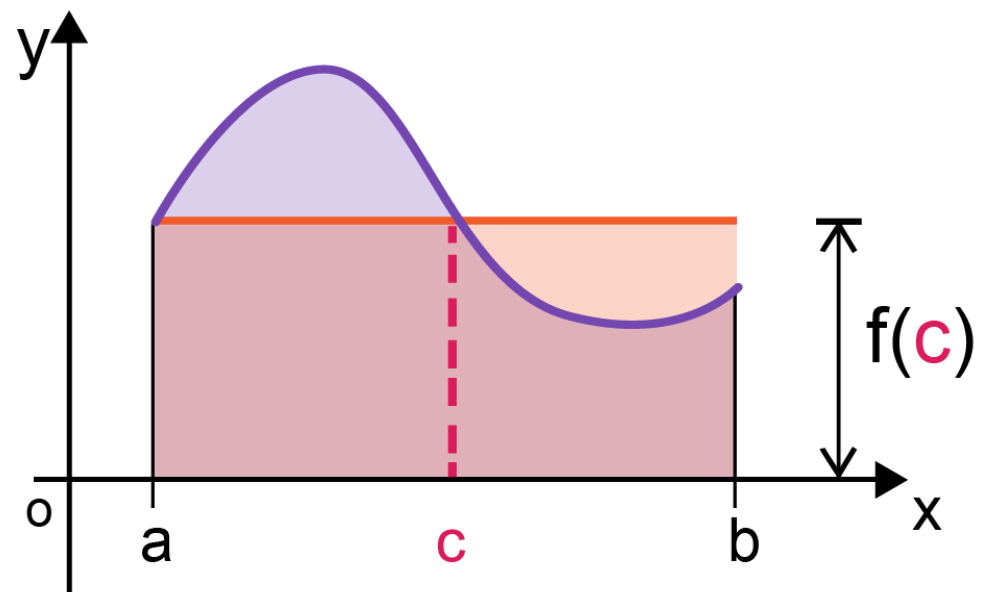
\includegraphics[width=0.4\linewidth]{08-mean-value}%
	\caption{Geometrický význam integrální věty o střední hodnotě.}
\end{figure}

\begin{proof}
	Položme $m = \min \{ f(x) \mid a \leq x \leq b \}$ a $M = \max \{ f(x) \mid a \leq x \leq b \} $
	Zřejmě
	\[ m(b-a) \leq \int_{a}^{b} f(x) \,dx \leq M(b-a) \]
	Existuje tedy $K$ takové, že $m \leq K \leq M$ a $\int_{a}^{b} f(x) \,dx = K(b-a)$.
	Jelikož $f$ je spojitá, existuje $c \in \left< a,b \right>$ takové, že $K = f(c)$.
\end{proof}

\subsection{Základní věta analýzy}
\begin{theorem}[Základní věta analýzy]
	Buď $f: \left< a,b \right> \to \mathbb{R}$ spojitá. Pro $x \in \left< a,b \right>$ definujeme
	\[ F(x) = \int_{a}^{x} f(t) \,dt \]
	Potom je $F'(x) = f(x)$
\end{theorem}

\begin{proof}
	Pro $h\neq 0$ máme
	\[ \frac{1}{h}(F(x+h) - f(x)) =\frac{1}{h}\left( \int_{a}^{x+h} f - \int_{a}^{x} f \right) =
	\frac{1}{h} \int_{x}^{x+h} f = \frac{1}{h}f(x + \theta h)h = f(x + \theta h) \]
	V druhé úpravě používáme úvahu $\int_a^b f+ \int_b^c f = \int_a^c f$ a ve třetí integrální větu o střední hodnotě.
\end{proof}

\begin{consequence}
	\hfill
	\begin{enumerate}
	    \item Spojitá funkce $f : \left<a,b\right> \rightarrow \mathbb{R}$ má na intervalu $(a,b)$ primitivní funkci spojitou na $\left<a,b\right>$.
	          Pro kteroukoli primitivní funkci $G$ funkce $f$ na $(a,b)$ spojitou na $\left<a,b\right>$ platí
	          \[\int^b_a f(t)dt = G(b) - G(a).\]
	    \item Integrální věta o střední hodnotě:
	    \[F(b) - F(a) = \int^b_a f = f(c)(b-a) = F'(c)(b-a)\]
	\end{enumerate}
\end{consequence}

\end{document}
